% Secondary Analyses, continued from secondary-analyses.tex.
\subsection{Demonstrated Extension Workflow}
\label{app:extension-workflow}

\begin{figure*}[htbp]
\floatconts
  {fig:benchmark}
  {\caption{\SLICES{} benchmark. The reusable path from fixed specification through objective extension and encoder transfer to auditable results. Comparison checks enforce declared settings and export coverage. They do not prove that a training run used its declared private data. Objective-specific modules and compute remain different.}}
  {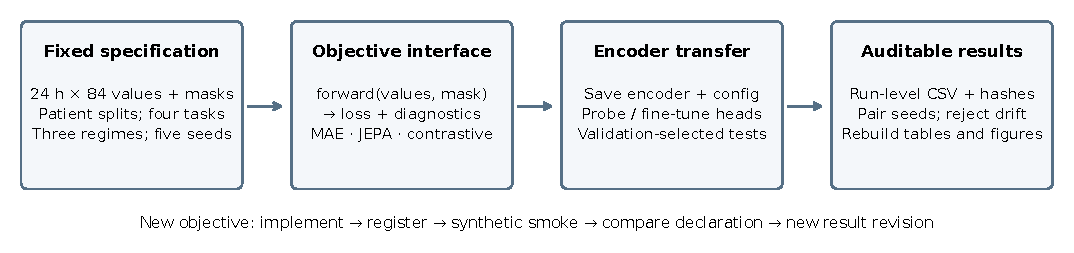
\includegraphics[width=\textwidth]{generated/benchmark-overview.pdf}}
\end{figure*}

The code repository's \texttt{TS2VEC\_CASE.md} gives a runnable path through the existing extension. Objective code, its configuration dataclass, registry entries, encoder-compatibility entry, and SSL YAML define the replaceable components. Clinical preprocessing, feature order, the shared encoder, final-epoch transfer, task heads, protocol schedules, primary metrics, and result identities define the retained scientific contract. The case adds execution and reporting code. It does not alter the objective or the archived results.

The command \texttt{extension.py --out extension-output} uses 80 artificial patients, the shared 70/15/15 split function, train-only normalization, and the full 159,808-parameter encoder. It runs two SSL epochs and two epochs for each synthetic binary/regression task under each protocol. These reduced budgets, artificial targets, and single seed are recorded as departures from the scientific contract. Checks cover exact v3 encoder transfer, discarded projection weights, unchanged frozen parameters, updated fine-tuned parameters, validation selection, and exact test-checkpoint reload. Synthetic metrics remain in a separate output file. The report on archived runs instead joins 120 existing TS2Vec runs to their matched core-contrastive runs, retaining means, sample SDs, paired differences, and configuration IDs.

Validation records distinguish implementation assistance and failed attempts from successful execution of the extracted archive's instructions. This is a development-agent check on a fresh environment, with no independent human reuse study. It does not test credentialed extraction, clinical label construction, or historical numerical retraining equivalence, which Appendix~\ref{app:reproduction} examines for a \MIMIC{} slice.

\subsection{Post-Hoc Random-Encoder Diagnostic}
\label{app:random}

The random diagnostic contains 40 task--dataset--seed rows over \MIMIC{} and \EICU{}. It freezes an untrained instance of the same default Transformer and trains only the linear task head from cached embeddings. Pairing those rows with the three core SSL probes gives 120 comparisons. The random probe is worse in 118. The exceptions are both against \JEPA{} on \EICU{}, by at most .001 AUPRC, for AKI and 24-hour mortality in one run each. This analysis was produced after the archived results and was not part of the core family. The raw/mask control below is another separate diagnostic.


\subsection{JEPA, Checkpoint, and Hyperparameter Diagnostics}
\label{app:diagnostics}

The separate JEPA diagnostic covers all 15 core pretraining runs. Across logged steps, the minimum target representation SD is .37 and the maximum mean pairwise cosine is .82. The mean final SD is 1.17. These statistics cannot rule out partial collapse or establish downstream quality. The historical checkpoint audit covers 45 core pretraining encoders. Core downstream runs use the final 100-epoch encoder. Retained JEPA validation-checkpoint files are from epochs 3--5. These are not final encoders and do not mean training ended early.

The checkpoint diagnostic completes 60 frozen probes, or 30 final-versus-best-SSL-validation pairs, over the three core objectives, five seeds, and MIMIC-IV hospital mortality and LOS. Both arms use the same cached CPU implementation, patient splits, train-only normalization, head initialization and batch RNG. Linear heads use the reference AdamW/cosine settings, validation patience and epoch cap. LOS trains with squared error and selects/reports absolute error. Validation alone selects the head, with the earliest epoch retained on a tie. The test set is evaluated once afterward. Producer checks matched all 30 encoder hashes to the archived encoder audit. The public audit reconstructs paired statistics and all 60 selections from saved validation histories.

\begin{table*}[htbp]
\floatconts{tab:checkpoint-sensitivity}
{\caption{Separate MIMIC-IV cached CPU probe diagnostic. Mean $\pm$ sample SD over five seeds. Mortality uses AUPRC. LOS uses absolute error in days. $\Delta$ is best-SSL-validation minus rerun-final. Brackets give the observed paired range. These final-arm values are reruns, not substituted historical scores.}}
{\scriptsize\begin{tabular}{llrlll}
\toprule
Task & Encoder & $n$ & Rerun final & Best SSL val. & $\Delta$ mean [range] \\
\midrule
Hospital mortality & MAE & 5 & 0.5093 $\pm$ 0.0135 & 0.5096 $\pm$ 0.0139 & +0.0003 [-0.0009, +0.0019] \\
Hospital mortality & JEPA & 5 & 0.4139 $\pm$ 0.0196 & 0.3733 $\pm$ 0.0094 & -0.0406 [-0.0563, -0.0166] \\
Hospital mortality & Contrastive & 5 & 0.4574 $\pm$ 0.0236 & 0.4573 $\pm$ 0.0236 & -0.0001 [-0.0003, +0.0000] \\
Remaining LOS & MAE & 5 & 2.7655 $\pm$ 0.0651 & 2.7644 $\pm$ 0.0628 & -0.0011 [-0.0047, +0.0019] \\
Remaining LOS & JEPA & 5 & 2.6758 $\pm$ 0.0903 & 2.9396 $\pm$ 0.0916 & +0.2638 [+0.1909, +0.3689] \\
Remaining LOS & Contrastive & 5 & 2.5946 $\pm$ 0.0662 & 2.5949 $\pm$ 0.0655 & +0.0003 [-0.0009, +0.0018] \\
\bottomrule
\end{tabular}
}
\end{table*}

JEPA worsens in all five seeds on both tasks (Table~\ref{tab:checkpoint-sensitivity}). For MAE and contrastive learning, the choice between final and best-validation encoders changes mean AUPRC and mean LOS error by at most .001 (AUPRC or days). MAE leads mortality and contrastive leads LOS under both policies in every seed, while JEPA's LOS mean rank drops from second to third. These LOS ranks use the capped squared-error probe, whose ordering did not survive loss matching (Section~\ref{sec:results}). The per-seed selections, validation histories, and paired differences are in \texttt{results/checkpoint-sensitivity/}, and \texttt{CHECKPOINT\_CASE.md} documents how to recompute them. Rerun-final cell means differ from historical means by at most .001 AUPRC and .01 LOS days. The largest absolute per-seed LOS deviation is .09 days. Cached CPU execution and dedicated paired RNG differ from historical GPU/Lightning execution. This diagnostic took about 20 wall minutes on CPU, with no failed or timed-out workers. It supports scoped checkpoint sensitivity, not equivalence, general rank stability, or conclusions about other databases or full fine-tuning.

Table~\ref{tab:hp} contains only MIMIC-IV 24-hour mortality, full fine-tuning, full labels, and five seeds per level. Learning-rate values are upstream pretraining rates. Mask sweeps change their respective objective's mask ratio. The largest within-sweep range of mean AUPRC is .018. This targeted slice establishes neither hyperparameter insensitivity nor objective-specific optimal tuning. Its test-set rankings are not used to select a new headline configuration.

\begin{table*}[htbp]
\floatconts{tab:hp}{\caption{Targeted pretraining hyperparameter diagnostics. Downstream AUPRC mean and sample SD, $n=5$ per level.}}
{\scriptsize\begin{tabular}{lllrr}
\toprule
Sweep & Objective & Level & AUPRC & SD \\
\midrule
lr sensitivity & Contrastive & 0.0002 & 0.462 & 0.035 \\
lr sensitivity & Contrastive & 0.0005 & 0.465 & 0.033 \\
lr sensitivity & Contrastive & 0.002 & 0.459 & 0.042 \\
lr sensitivity & JEPA & 0.0002 & 0.467 & 0.028 \\
lr sensitivity & JEPA & 0.0005 & 0.461 & 0.049 \\
lr sensitivity & JEPA & 0.002 & 0.449 & 0.053 \\
lr sensitivity & MAE & 0.0002 & 0.462 & 0.047 \\
lr sensitivity & MAE & 0.0005 & 0.451 & 0.051 \\
lr sensitivity & MAE & 0.002 & 0.457 & 0.050 \\
mask ratio sensitivity & JEPA & 0.3 & 0.454 & 0.057 \\
mask ratio sensitivity & JEPA & 0.75 & 0.447 & 0.029 \\
mask ratio sensitivity & MAE & 0.3 & 0.464 & 0.033 \\
mask ratio sensitivity & MAE & 0.75 & 0.447 & 0.035 \\
view mask sensitivity & Contrastive & 0.3 & 0.460 & 0.035 \\
view mask sensitivity & Contrastive & 0.75 & 0.447 & 0.061 \\
\bottomrule
\end{tabular}
}
\end{table*}

\subsection{Raw-Input and Mask-Only CPU Control}
\label{app:raw}

This post-hoc diagnostic uses only MIMIC-IV hospital mortality and the five canonical patient splits. A linear logistic classifier receives either 2,016 flattened mask entries or those entries plus 2,016 normalized values. Normalization uses the same full-cohort training partition. Task labels are filtered after patient assignment. Fixed SGD uses logistic loss, $L_2$ coefficient $10^{-4}$, the library's optimal learning-rate schedule, square-root-balanced sample weights, and 20 epochs. The epoch with highest validation average precision is evaluated once on the test set. No label smoothing or hyperparameter search is used. The implementation and input-file SHA256 values are recorded separately.

Test AUPRC is .301 (.025) for masks and .404 (.013) for values plus masks, mean (sample SD). Mean test support is 11,157 stays and 1,310 deaths. Total wall time is 136 seconds on a CPU limited to two threads, including both representations and all five seeds, under a 900-second hard timeout. Every mask-only run selects epoch 20, so further optimization could improve this control. The result does not establish the performance of an optimized raw-input model, nor does it isolate SSL gains from differences in optimization, regularization, input dimension, or head training.
